\cotefile{53}
\scanpage{16}
\[
\left\{\begin{aligned}
&\text{Groupes sur des bases } S\ \text{quelconques. Prendre base } S\ \deleted{\unsure{?}}\ \text{ou prendre base } k\ \text{?}\\
&\text{Groupes \unsure{non-affines|n.-affines} O.K.}
\end{aligned}\right.
\]

Représentations linéaires des $D(M)$ [cas particuliers : $\unsure{\mathbb{G}_m|G_m}$, $\mu_n$]

Application : homomorphismes $D(M)\longrightarrow\mathbb{G}_m$ : on trouve que $M_S$ est ``réflexif'' vis à vis de $\mathbb{G}_m$.

\uline{Dualité de Cartier}\quad $\underline{\mathrm{Hom}}(G,\mathbb{G}_m)$ \deleted{\unsure{$\overset{\Delta}{=}$|est}} représentable ? Cela l'est si $G$ diagonalisable, mais \deleted{pas}\inserted{en général (\unsure{=|ex.|i.e.} pour $G=\mathbb{G}_m$)} pour un schéma en groupes affine (\unsure{même} de t.f.). Par contre, si $G$ est fini loc. libre sur $S$, on a
% slanted
\reversemarginpar\margin{$\underline{\mathrm{Hom}}_{\mathrm{gr}}(G,H)$ représentable si $G$ est fini loc. libre, $H$ affine (disons)}\normalmarginpar
\[
\underline{\mathrm{Hom}}_{\mathrm{gr}}(G,\mathbb{G}_m)
\subset \mathrm{Hom}_{\unsure{\mathcal O|O|\mathbb O}\text{-alg}}
(\mathcal O_S[T,T^{-1}],\unsure{\mathcal A|A})\simeq W(\mathcal A)^*,
\]
et le sous foncteur est celui des \deleted{$\unsure{g}$} $u\in W(\mathcal A)^*(S')$ tels que
\[
\unsure{\Pi|\Delta}(u)=u\otimes u\qquad \varepsilon(u)=1
\]
\margin{[\,\uline{NB} On peut donc oublier la condition $u$ inv. car $\underline{\mathrm{Hom}}_{\mathrm{gr}}(G,\mathbb{G}_m)=\underline{\mathrm{Hom}}_{\unsure{\mathrm{mon}}}(G,\mathcal O^{\unsure{\times|*}})$.}

\deleted{\unsure{La}} La représentabilité est claire, mais de plus on reconnaît que c'est \deleted{\unsure{le|à}} $\mathrm{Spec}(\check{\mathcal A})$, $\check{\mathcal A}$ \deleted{étant}\inserted{$=\underline{\mathrm{Dist}}(G)_{\unsure{/S|S}}$} une algèbre grâce à la structure de coalgèbre de $\mathcal A$. D'autre part, la structure de coalgèbre de $\check{\mathcal A}$ (provenant du fait que le foncteur qu'il représente est un foncteur-groupe
% slanted
\reversemarginpar\margin{$\check{\mathcal A}$ comm. car $G$ l'est. Si $G$ n'est pas comm., il faut prendre le foncteur $k'\longmapsto\mathrm{Hom}_{\unsure{k\text{-alg}}}(\check{\mathcal A},k')=\mathrm{Hom}_{k\text{-alg}}({\check{\mathcal A}\deleted{\unsure{)}}}_{\unsure{\mathrm{ab}}},k')$}\normalmarginpar

\uline{Th.} Tout groupe comm. fini loc. libre \inserted{$G$} est réflexif pour
\par\noindent\begin{tabular}{@{}|p{.91\linewidth}@{}}
$\mathbb{G}_m$. Son dual $G^*$ est fini loc. libre comm., d'où une \uline{\unsure{d'involution|involution}} $G\unsure{\mathrel{\vert\!-\!{\cdot}}|\mapsto}G^*$ de la catégorie des groupes comm. loc. libres. Elle correspond à la dualité des bialgèbres bicommutatives sur $S$.
\end{tabular}

\[
\begin{aligned}
\text{\uline{Ex}}\qquad &\mu_n\longleftrightarrow\mathbb Z/n\mathbb Z
&\ \Bigg|\, &\text{Mais aussi }\ D(M)\longleftrightarrow M_S\\
&\alpha_p\longleftrightarrow\alpha_p && 
\end{aligned}
\]

Marche $\pm$ pour les schémas en groupes \deleted{\unsure{affines}} \deleted{\illegible{1}} sur $S$ \deleted{\unsure{tel que|tels que}\ldots}\inserted{qui} se dévissent en groupes finis loc. libres, groupes discrets, groupes diagonalisables, et versions \deleted{\unsure{discre|discrè}} tordues\ldots\ Si on veut inclure le groupe $\mathbb{G}_a$, il faut \ldots

La dualité de Cartier domine la théorie des groupes algébriques \unsure{(ou} formels) commutatifs, affines ou non -- mais il faut la complémenter par \unsure{considération|la considération} des $\underline{\mathrm{Ext}}^1(G,\mathbb{G}_m)$ alors.
% archive sheet number: 15
\clearpage
\scanpage{17}
% Isolated opaque stroke to the left of the date.
\figure{
\begin{tikzpicture}[x=1mm,y=1mm]
\fill (0,.4)--(.5,3.3)--(2.3,2.6)--(5,2.2)--(8.1,1.1)--(11,.3)--(10.7,-1.2)--(8.1,-.5)--(4.7,.2)--(2,.6)--(.8,0)--cycle;
\end{tikzpicture}}
\hfill June 15, 1973.\\
Prof Grothendieck,\\

The last proposition stated in the course on alg groups was\unsure{\textsuperscript{-}|\textsuperscript{,}}

``\uline{Prop}: If $k$ is a field, $G$ an affine alg\unsure{,|.} monoid (resp, an affine alg group).

a) $G=\varprojlim G_i$\qquad where each $G_i$ is an affine alg monoid of finite type over $k$. (resp, affine alg. group of finite type over $k$).

b) If $G$ is of finite type, $\exists$ a closed immersion (of monoids).
\[
G\hookrightarrow\unsure{.}\ \mathrm{GL}(\unsure{n|u})_k\ \unsure{\text{''}|{}^{u}}
\]

I still see difficulty in accepting b). The closed immersion of monoids corresponds to a surjective mapping of coalgebras
\diagram{\begin{minipage}[t]{.39\linewidth}\vspace{0pt}\centering
\begin{tikzcd}[ampersand replacement=\&,column sep=large]
 A \& B\arrow[l,two heads]
\end{tikzcd}
\end{minipage}\hfill
\begin{minipage}[t]{.51\linewidth}\vspace{0pt}
$B$ an algebra representing\\
$\mathrm{GL}(n)$\par
$A$ an algebra representing\\
$G$,
\end{minipage}}

$B$ has an antipodal map (corresponding to the ``inverse'' map in the on the group object in the cat. $\mathrm{Aff}_k$\unsure{.})
% archive sheet number: 16
\clearpage
\scanpage{18}
\mspage{- 2 -}
\figure{
\begin{tikzpicture}[x=1mm,y=1mm]
\fill (0,2.5)--(1.5,3.1)--(4.1,2.8)--(5.5,2.1)--(7.3,1.9)--(9.2,.6)--(8.7,-.3)--(6.1,.15)--(2.5,.5)--cycle;
\end{tikzpicture}}

the surjectivity $B\twoheadrightarrow A$ will induce the antipodal map on the $k$-algebra $A$ and thus ``force'' it to be a group object (not the more general monoid object) in $\mathrm{Aff}_k$.

Consider the example
\[
\begin{aligned}
\{0,1\}: \mathrm{Alg}_k&\longrightarrow\mathrm{Sets}\\
k'&\longmapsto\mathrm{Hom}_{k\text{-alg}.}(k\times k,k').
\end{aligned}
\]

Make $A=k\times k$ into a coalgebra over $k$ by
\[
\begin{aligned}
 A&\xrightarrow{\unsure{\Pi_0|\pi_0|\Pi_o|\pi_o}}A\otimes A\\
 (a,b)&\longmapsto\unsure{.}\ (a,b)\otimes(1,0)+(1,1)\otimes(0,b).
\end{aligned}
\]

the two projections\unsure{.}
\[
\begin{aligned}
\unsure{P|p}_1 &: (a,b)\longmapsto a.\\
P_2 &: (a,b)\longmapsto b
\end{aligned}
\]
represent $k$-valued points of $\{0,1\}$

multiplication table :
\diagram{$\begin{array}{c|cc}
\Pi & P_1 & P_2\\ \hline
P_1 & \multicolumn{1}{c|}{P_1} & P_2\\ \cline{2-3}
P_2 & \multicolumn{1}{c|}{P_2} & P_2
\end{array}$}

(this is easy to check :
\[
\begin{aligned}
(P_1,P_1)&:(a,b)\otimes(c,d)&\longmapsto\unsure{ac|\acute a\acute c|a'c'}\unsure{.}\\
(P_1,P_2)&:\qquad\text{\rq\rq}&\longmapsto ad\\
(P_2,P_1)&:\qquad\text{\rq\rq}&\longmapsto bc\\
(P_2,P_2)&:\qquad\text{\rq\rq}&\longmapsto bd.
\end{aligned}
\]
% archive sheet number: 17
\clearpage
\scanpage{19}
\mspage{- 3 -}
\figure{
\begin{tikzpicture}[x=1mm,y=1mm]
\fill (0,0)--(.6,1.3)--(.7,3)--(3.4,1.8)--(7.6,.6)--(7.5,-.4)--(3.4,.1)--cycle;
\end{tikzpicture}}

so that
\[
\begin{aligned}
(\unsure{P|p}_1,P_1)\circ\unsure{\Pi_0|\pi_0|\Pi_o|\pi_o}&=P_1\\
(P_1,P_2)\circ\Pi_0&=P_2\\
(P_2,P_1)\circ\Pi_0&=P_2\\
(P_2,P_2)\circ\Pi_0&=P_2.
\end{aligned}
\]

It is easy to check that $P_1:A\otimes A\longrightarrow k$ is a counit, that $\Pi_0$ is co-associative, co-commutative.
\margin{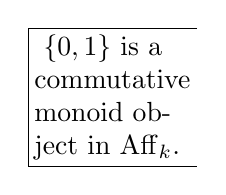
\begin{tikzpicture}[baseline=(note.base)]
\node[anchor=north west,align=left,text width=1.99cm,inner sep=2pt] (note) at (0,0)
{$\therefore\ \{0,1\}$ is a commutative monoid object in $\mathrm{Aff}_k$.};
\draw (note.north east)--(note.north west)--(note.south west)--(note.south east);
\end{tikzpicture}}

But $\{0,1\}(k)$ can't be a group object in sets.
\[
\begin{aligned}
&\text{\rq\rq}\\[-2pt]
&\{P_1,P_2\}.
\end{aligned}
\]

Moreover $A$ can't be given a co-inversion or antipodal map. One way of characterizing the inverse \inserted{$\sigma$} for \unsure{commut|commut.} gps is that $\exists\,\sigma:G\longrightarrow G$ \unsure{sud|such} that
\diagram{\begin{minipage}[t]{.47\linewidth}\vspace{0pt}\centering
\begin{tikzcd}[ampersand replacement=\&,row sep=large,column sep=small]
G\arrow[r,"{\unsure{I_G|1_G}\times\sigma}"] \&
G\times G\arrow[d,"\Pi","{\unsure{\cdot}}"{pos=.92,swap},"{\unsure{\cdot}}"{pos=.94}]\\
\& G
\end{tikzcd}
\end{minipage}\hfill
\begin{minipage}[t]{.48\linewidth}\vspace{0pt}
factors through the final then initial object :
\end{minipage}}
\diagram{\begin{tikzcd}[ampersand replacement=\&,row sep=2pt,column sep=3pt]
G\arrow[rr,"{I_G\times\sigma}"]\arrow[ddd] \& \& G\times G\arrow[ddd,"\Pi"] \& \&
 \text{i.e. that\unsure{.}}\arrow[dl,bend left=15]\\
\& {x\longmapsto(x,x^{-1})}\arrow[d,maps to] \& \& \vphantom{G} \&
 \begin{gathered}\text{commutes since}\\\text{the final }+\text{ initial}\\\text{objs coincide.}\end{gathered}\\
\& e.\& \& \&\\
e\arrow[rr,"{\unsure{\cdot}}"{pos=.94,below}] \& \& G \& \&
\end{tikzcd}}
% archive sheet number: 18
\clearpage
\scanpage{20}
\mspage{- 4 -}
\figure{
\begin{tikzpicture}[x=1mm,y=1mm]
\fill (0,0)--(1.1,.7)--(1.2,2.1)--(3.7,1.7)--(6.3,1.1)--(7.4,.2)--(7.5,-.4)--(3,.1)--cycle;
\end{tikzpicture}}

On the coalgebra level $\exists\ A\xrightarrow{\unsure{\sigma_0|\sigma_o}} A$\quad s.t.
\diagram{\begin{minipage}[t]{.43\linewidth}\vspace{0pt}\centering
\begin{tikzcd}[ampersand replacement=\&,row sep=large,column sep=large]
 A \& A\otimes A\arrow[l,"{\unsure{I_A|1_A}\otimes\sigma_0}"']\\
 k\arrow[u,"\text{structure}" description] \& A\arrow[l,"\text{counit}"]\arrow[u,"{\unsure{\Pi_0|\pi_0|\Pi_o|\pi_o}}"']
\end{tikzcd}
\end{minipage}\hfill
\begin{minipage}[t]{.54\linewidth}\vspace{0pt}\small
Suppose $\sigma_0$ exists in this case :
\[
\sigma_0(c,d)=(\sigma_{01}(c,d),\sigma_{02}(c,d)).
\]
Where\unsure{.}
\[
\sigma_{0i}=\unsure{P|p}_i\circ\sigma_0.
\]
\end{minipage}}

\diagram{\begin{minipage}[t]{.55\linewidth}\vspace{0pt}
Now compute : the lower left route gives :
\end{minipage}\hfill
\begin{minipage}[t]{.42\linewidth}\vspace{0pt}\centering
\begin{tikzcd}[ampersand replacement=\&,column sep=small]
{(a,a)} \& \\
a\arrow[u,maps to,"{\text{structure\unsure{.}}}" description] \& {(a,b)}\arrow[l,maps to,"{P_1}"]
\end{tikzcd}
\end{minipage}}

\unsure{the|The} upper right route gives :
\diagram{\footnotesize\begin{tikzcd}[ampersand replacement=\&,column sep=small,row sep=small]
{(a,b)\cdot(\sigma_{01}(1,0),\sigma_{02}(1,0))} \& {(a,b)\otimes(1,0)+(1,1)\otimes(0,b)}\arrow[l,maps to]\\
{+} \&\\
{(1,1)\cdot(\sigma_{01}(0,b),\sigma_{02}(0,b)\unsure{{}^{\prime}|{\cdot}}} \& {(a,b)}\arrow[uu,maps to]
\end{tikzcd}}
\[
\begin{aligned}
&\unsure{\text{\rq\rq}|\shortparallel}\\
&\bigl(a\sigma_{01}(1,0)+\sigma_{01}(0,b),\
 b\sigma_{02}(1,0)+\sigma_{02}(0,b)\unsure{.}\bigr)
\end{aligned}
\]

This above is to be equal to $(a,a)$ for all $(a,b)$ ? Perhaps I am very confused! or perhaps $\mathrm{GL}(\unsure{n|u})_k$ \deleted{could}\inserted{should} be changed to $\unsure{\mathcal E\mathit{nd}|\mathrm{End}}_k(M)$.

I'm enjoying the courses very much. Many thanks for letting me attend.\\
\hfill\unsure{F J|L J|E J|F. J.} \unsure{Servedio|Servedis}\\
\hfill Dalhousie U., Halifax, N.S.\\
% archive sheet number: 19
\clearpage
\scanpage{21}
\figure{
\begin{tikzpicture}[x=1mm,y=1mm]
\fill[gray] (-20.2,1.65) circle (.1);
\fill (-4.3,-.55) circle (.18);
\draw[gray,very thin] (-4.1,-.48)--(-.7,-.08);
\fill (0,0)--(.4,.65)--(2.8,1.55)--(5.65,2)--(6.3,1)--(7.1,.35)--(6.3,.2)--(4.8,.5)--cycle;
\end{tikzpicture}}

\begin{center}Prof Grothendieck\hspace{1.6em}\unsure{.}\end{center}

\figure{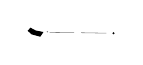
\begin{tikzpicture}[x=1mm,y=1mm]
\fill (0,.4)--(.35,.8)--(1,.45)--(2,.25)--(1.6,-.35)--(.5,-.05)--cycle;
\draw[gray,very thin] (2.8,.2)--(5.9,.16) (6.8,.16)--(10,.1);
\fill[gray] (2.5,.29) circle (.09);
\fill (10.9,.1) circle (.15);
\end{tikzpicture}}

\figure{\begin{tikzpicture}[x=1mm,y=1mm]
\draw[gray,very thin] (.2,.9) to[bend right=35] (.2,0);
\fill (10.9,.8)--(11.3,1.2)--(12,.9)--(11.85,.5)--(11,.55)--cycle;
\end{tikzpicture}}
% archive sheet number: 20.
\clearpage
\scanpage{22}
\uline{Rectification} \quad Si $G$ monoïde affine de t.f. sur corps $k$, on a une immersion fermée \unsure{multiplicatif|multiplicative} $G\unsure{\mathbin{-}|\longrightarrow}\unsure{M|\mathbb M}_{\unsure{n,k|n\,k}}$ (non $G\to\unsure{GL_{n,k}|Gl_{n,k}|GL(n,k)}$\unsure{)} car on peut montrer que si $G$ est un monoïde de \unsure{prés.|pres.} finie sur un anneau $k$, tel que les translations à g (disons sont des mono) - p.ex. s'il $\exists$ \unsure{mono|un} $G\longrightarrow G'$, $G'$ un \inserted{\unsure{foncteur en}} groupes - alors $\deleted{\unsure{G}}G$ est un \unsure{objet-groupe|objet groupe}).

\figure{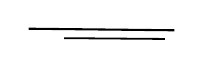
\begin{tikzpicture}[x=1cm,y=1cm]
\draw[line width=.75pt] (0,0) -- (1.85,-.02);
\draw[line width=.65pt] (.45,-.12) -- (1.73,-.13);
\end{tikzpicture}}

\deleted{\unsure{$G$|Soit}} $X$ schéma affine sur $k$, \deleted{\unsure{de|et}} de $k$-algèbre $\unsure{\mathcal A|A}$. On définit $\check{\mathcal A}=\mathrm{Dist}(X\deleted{\unsure{)|,}},k)$. On \unsure{a|.} le foncteur $\inserted{k'}\rightarrow\mathrm{Dist}(X,k')$, noté $\mathrm{Dis}(X)$, représentable par $\unsure{\mathbb V|V}(A)$. On a
% slanted
\reversemarginpar\margin{\tikz[baseline=-.3ex,x=1em,y=1em]{\draw[->] (.56,.85) to[out=-130,in=76] (0,-.55);} \uline{covariant}}\normalmarginpar
\[
\left\{\begin{aligned}
&\text{a)}\ \mathrm{Dist}(X)\ \text{fonctoriel en }X\quad
  (\text{comme Module sur }\unsure{\mathcal O|O}_k)\\
&\text{b)}\ \mathrm{Dist}(X)\times\mathrm{Dist}\unsure{Y)|(Y)}
  \xrightarrow[\unsure{\pi|\Pi}_{X,Y}]{\deleted{\unsure{\alpha|o}}}
  \mathrm{Dist}(X\times Y)\quad\text{bilinéaire}
\end{aligned}\right.
\]
[et universel pour les hom bilinéaires de $\mathrm{Dis}(X)\times\mathrm{Dis}(Y)$ dans un $\mathbb V(M)$] \unsure{induisant|induisent} en fait un \unsure{isom|isom.}
\[
\mathrm{Dist}(X)\boxtimes\mathrm{Dist}(Y)\simeq\mathrm{Dist}(X\times Y).
\]

c) On a une inclusion fonctorielle
\[
X\xrightarrow{\alpha_X}\mathrm{Dist}(X)
\]
[distribution ponctuelle, compatible avec passage au produit, i.e. on a comm. \unsure{des|du}
\diagram{\begin{tikzcd}[ampersand replacement=\&]
X\times Y \arrow[r,"\alpha_X\times\alpha_Y"] \arrow[dr,swap,"\unsure{\pi_{X\times Y}|\pi_{X,Y}}"] \& \unsure{\mathrm{Dist}}(X)\times\mathrm{Dist}(Y) \arrow[d,"\pi_{X,Y}"]\\
\& \mathrm{Dist}(X\times Y)
\end{tikzcd}}

\deleted{Si $G$ est muni d'une loi de comp., $\mathrm{Dist}(G)$ aussi. \deleted{\unsure{Si}} Elle est unitaire \unsure{sss|ssi} celle de $\mathrm{Dist}(G)$ l'est} En fait on peut \unsure{rêconstruire|réconstruire|reconstruire} $X$ à partir de $\mathrm{Dist}(X)=\unsure{\mathbb D|D}$ et la structure supplémentaire
\[
D\overset{\Delta}{\unsure{\mathbin{-}|\longrightarrow}}D\boxtimes D
\]
\margin{$[\,V(A)\boxtimes V(B)\overset{\text{déf}}{\simeq}V(A\otimes B)\,]$\newline
[NB $\boxtimes=\otimes$ si $A$ ou $B$ \unsure{proj.|proj} de t.f.]}
% slanted
\reversemarginpar\margin{NB on \unsure{réconstitue|reconstitue} $X$ à partir de $D$ muni \deleted{\unsure{la|du}}de l'application diagonale $D\to D\boxtimes\inserted{\unsure{D}}$ comm. ass. unitaire.}\normalmarginpar
doit être une ``application diagonale'' ass. comm. et counitaire [i.e. on a $D\xrightarrow{\unsure{\varepsilon|\epsilon}}\mathcal O$ \ldots.] comme formé des \deleted{\unsure{pts|gts}} $x\in\mathbb D(k')$ tels que
\[
\boxed{\Delta(x)=x\boxtimes x}
\]
% archive sheet number: 21
